\documentclass[../PS6_RapportFinal.tex]{subfiles}

\begin{document}
\graphicspath{{img/}{tex/img/}}
\subsection{Analyse de l'existant}
\label{analyseexistant}

L'analyse des différents échangeurs qui ont été conçus cette année ainsi que l'année dernière nous permet de mieux comprendre les apports des prototypes proposés. La première analyse effectuée cette année nous a permis de mettre en évidence des défauts dans la réaction de compostage. En effet, nous nous sommes rendu compte, en vidant la cuve, que la réaction n'avait eue lieu qu'au fond de cette dernière, où le compost était le plus dense. Les pertes étaient donc importantes, dans la mesure où plus de 80\% du volume de matière présente initialement n'avait pas réagi. De plus, l'idée de mettre un serpentin était discutable, puisqu’il fallait l'enlever de la cuve dès que l'on voulait changer le compost. Il s'agissait donc de trouver une solution facilitant cette opération.

\begin{figure}[!h]
\begin{center}
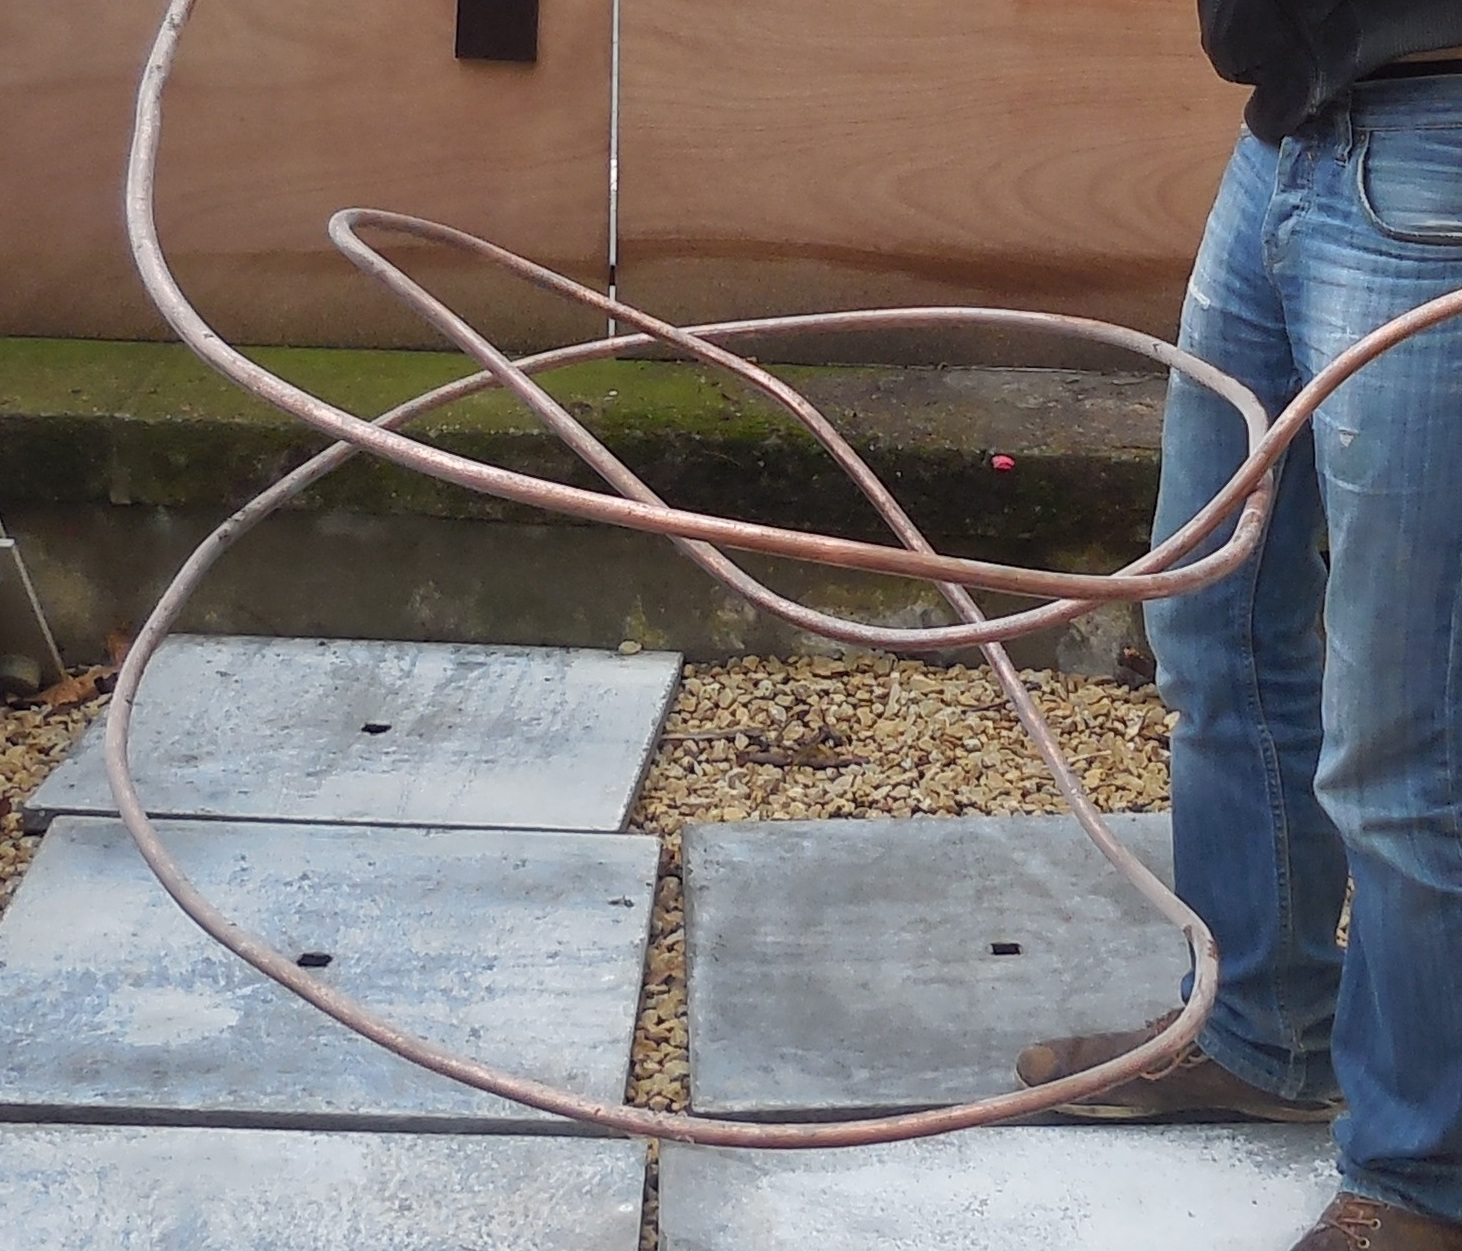
\includegraphics[scale=0.5]{3_1_Serpentin.JPG}
\caption{Illustration du serpentin utilisé l'année dernière}
\end{center}
\end{figure}

Il fallait ensuite étudier le raccordement au réseau hydraulique : les raccords existants induisaient des fuites non négligeables, et ainsi des pertes énergétiques, puisqu'ils n'étaient pas adaptés à la pression du réseau. Ceux que nous proposons actuellement corrigent ce défaut.

\begin{figure}[!h]
\begin{center}
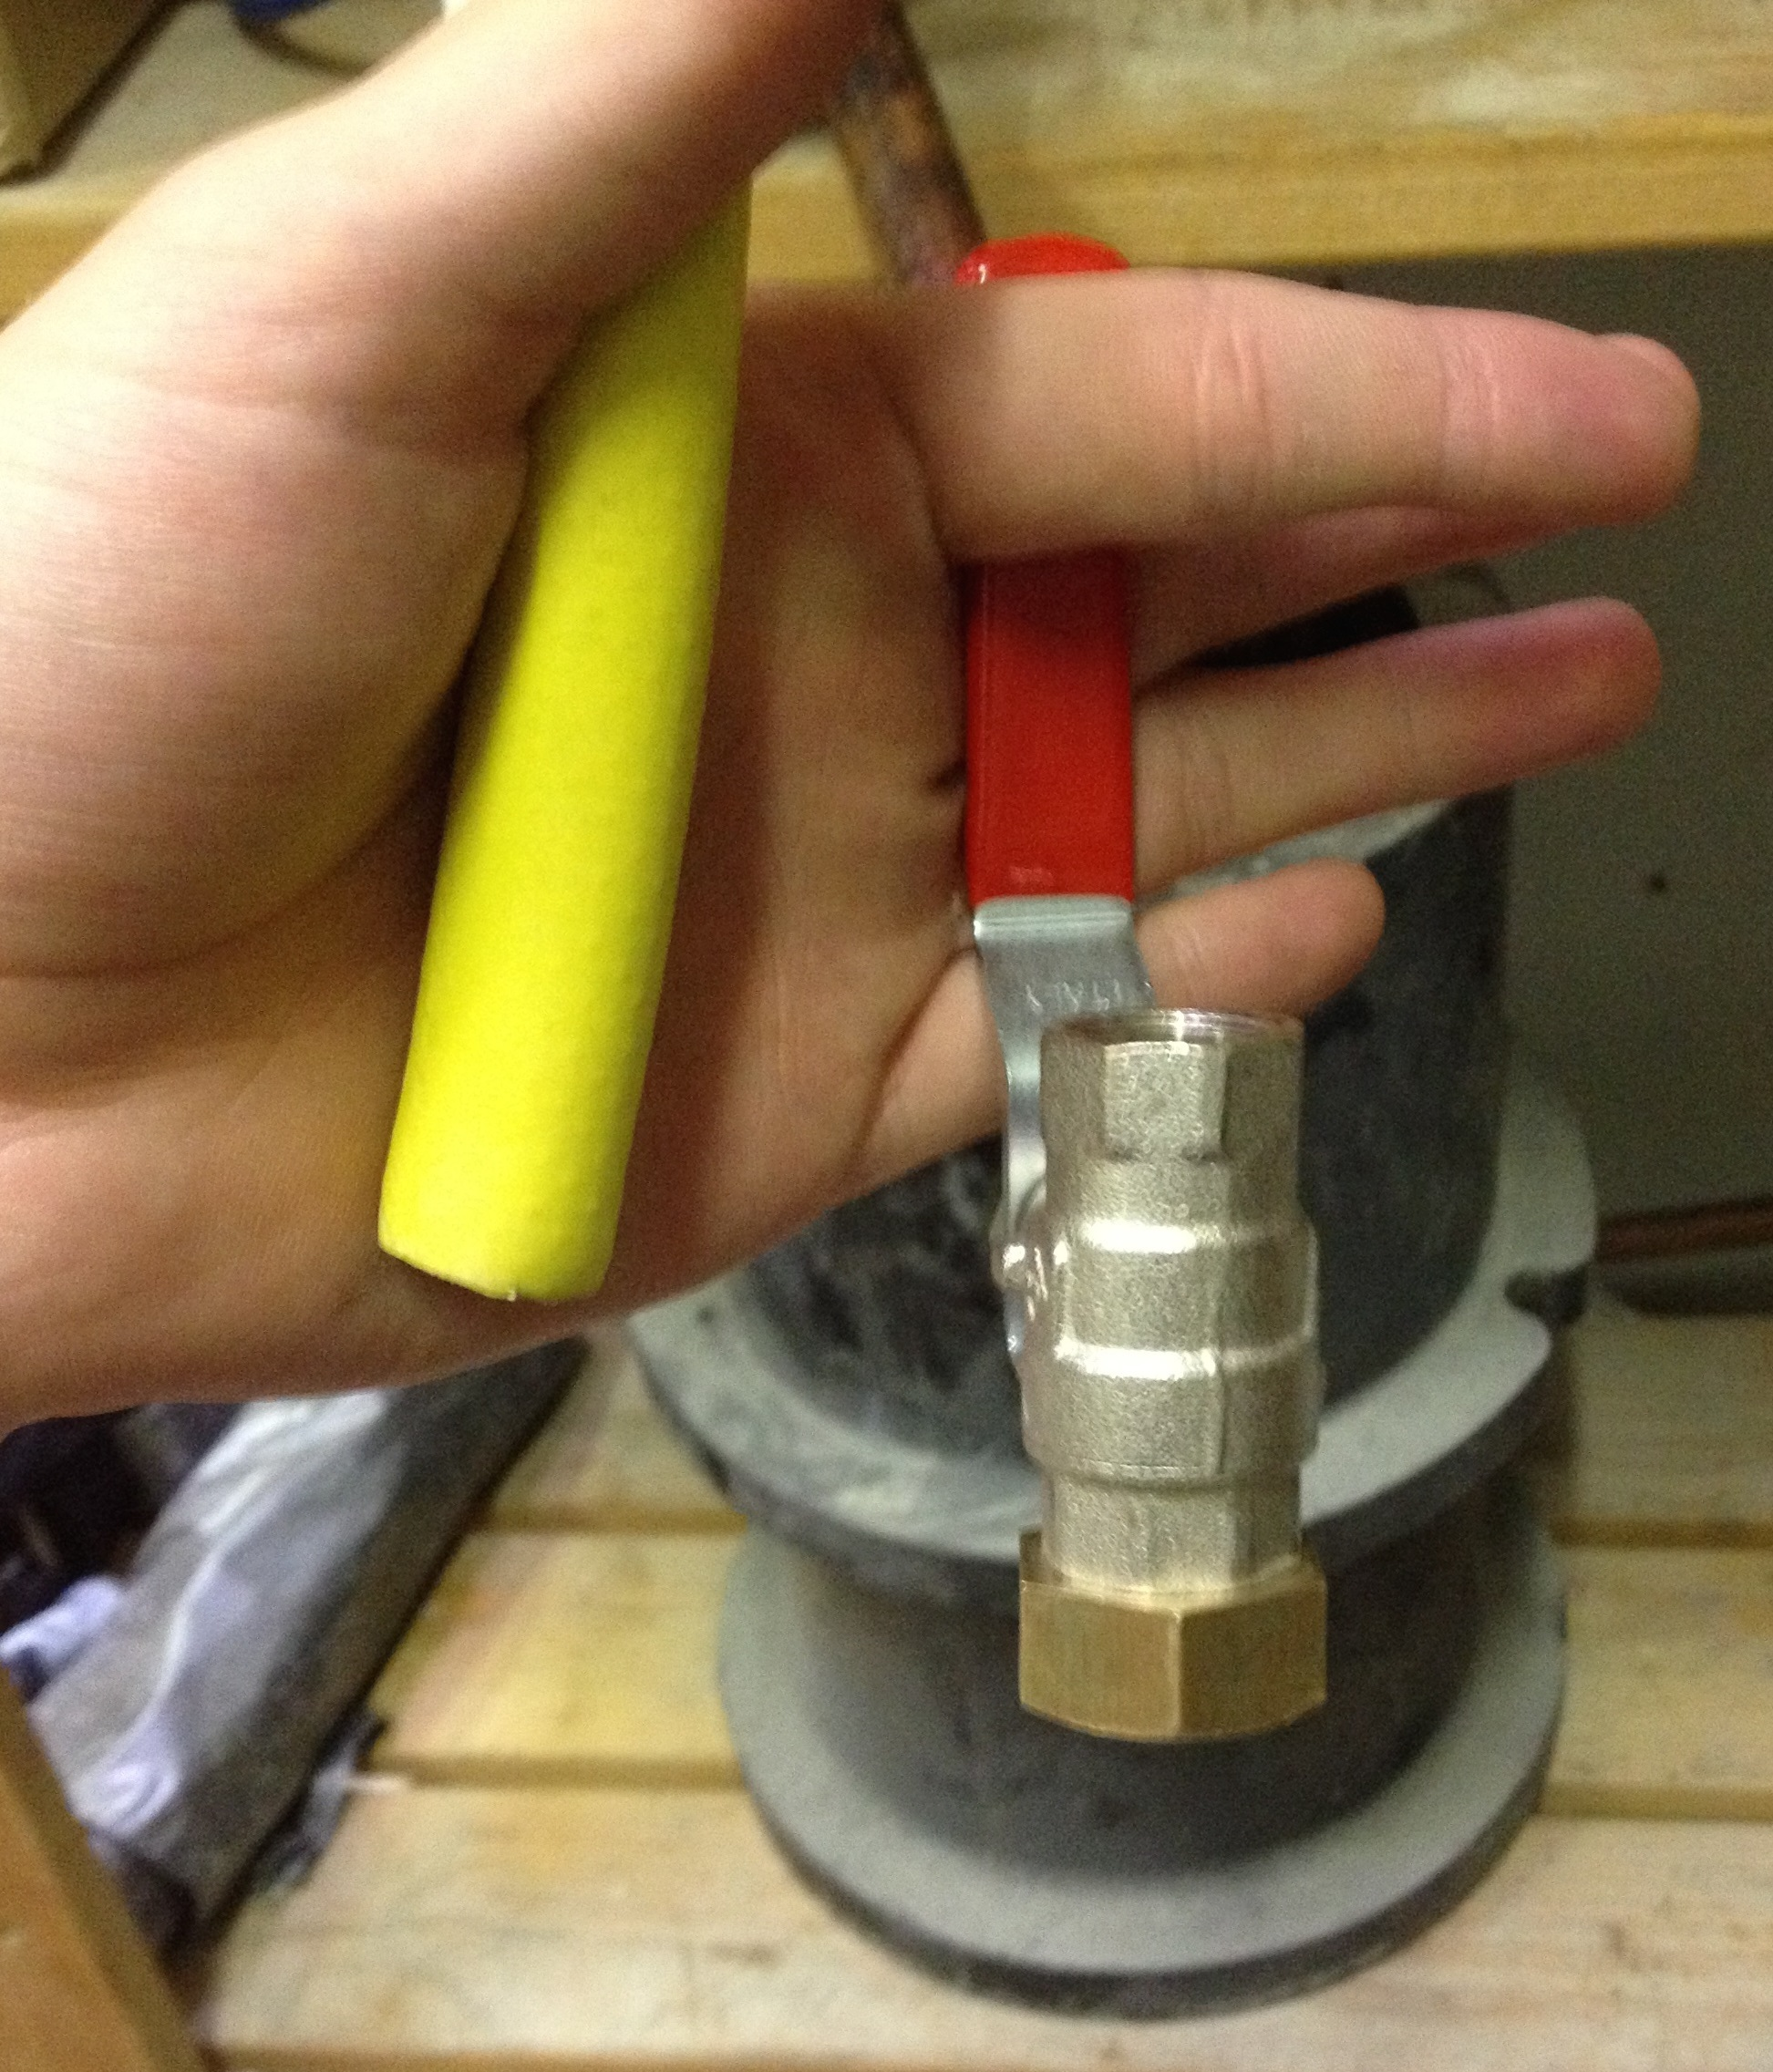
\includegraphics[scale=0.06]{3_1_Anciens_raccords.JPG}
\caption{Anciens raccords de l'échangeur}
\end{center}
\end{figure}

%\begin{figure}[h!]
%\begin{center}
%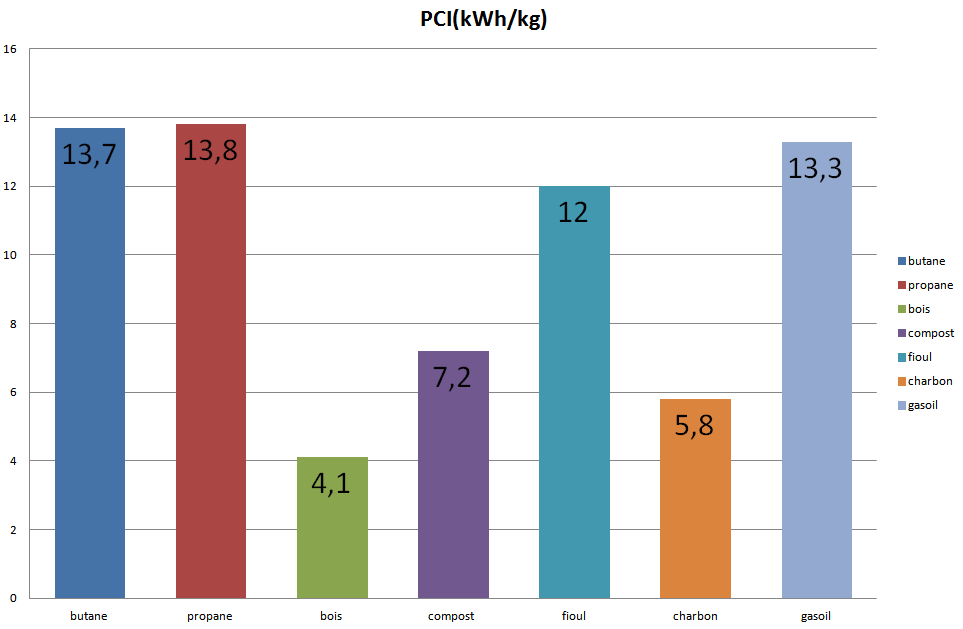
\includegraphics[scale=0.5]{1_2_Graphique_comparaison_energie.png}
%
%\end{center}
%\end{figure}
%(Ici photo 3.1.1. Légende = « Isolation des tubes à l’aide de joints et de colle »)

Enfin, un dernier constat quant à la réaction et ses pertes a été fait : celle ci était très largement privilégiée autour des tubes d’aération. Le système de pieux que nous proposons permet de limiter ces pertes puisque nous occupons un volume beaucoup plus important et bien plus homogène de compost. En plus de catalyser la réaction, nous récupérons par ailleurs une quantité plus importante d’énergie.
De plus, ce système s'appuie sur une technologie que nous souhaitions introduire cette année, à savoir celle des caloducs : ce sont des tubes qui permettent le transport de chaleur grâce au principe de l'équilibre entre deux phases. En effet, dans le tube se trouve un fluide  basse pression (afin d'avoir une température d'ébullition relativement faible) : dans la partie basse, celui-ci est en phase liquide tandis que dans la partie haute, il est en phase gazeuse. La fraction liquide est en fait chauffé jusqu'à évaporation par la source chaude, remontant ainsi et se condensant au niveau de la partie haute suite à un échange de chaleur avec la source froide, pour finalement redescendre sous l'action de la pesanteur.


\begin{figure}[!h]
\begin{center}
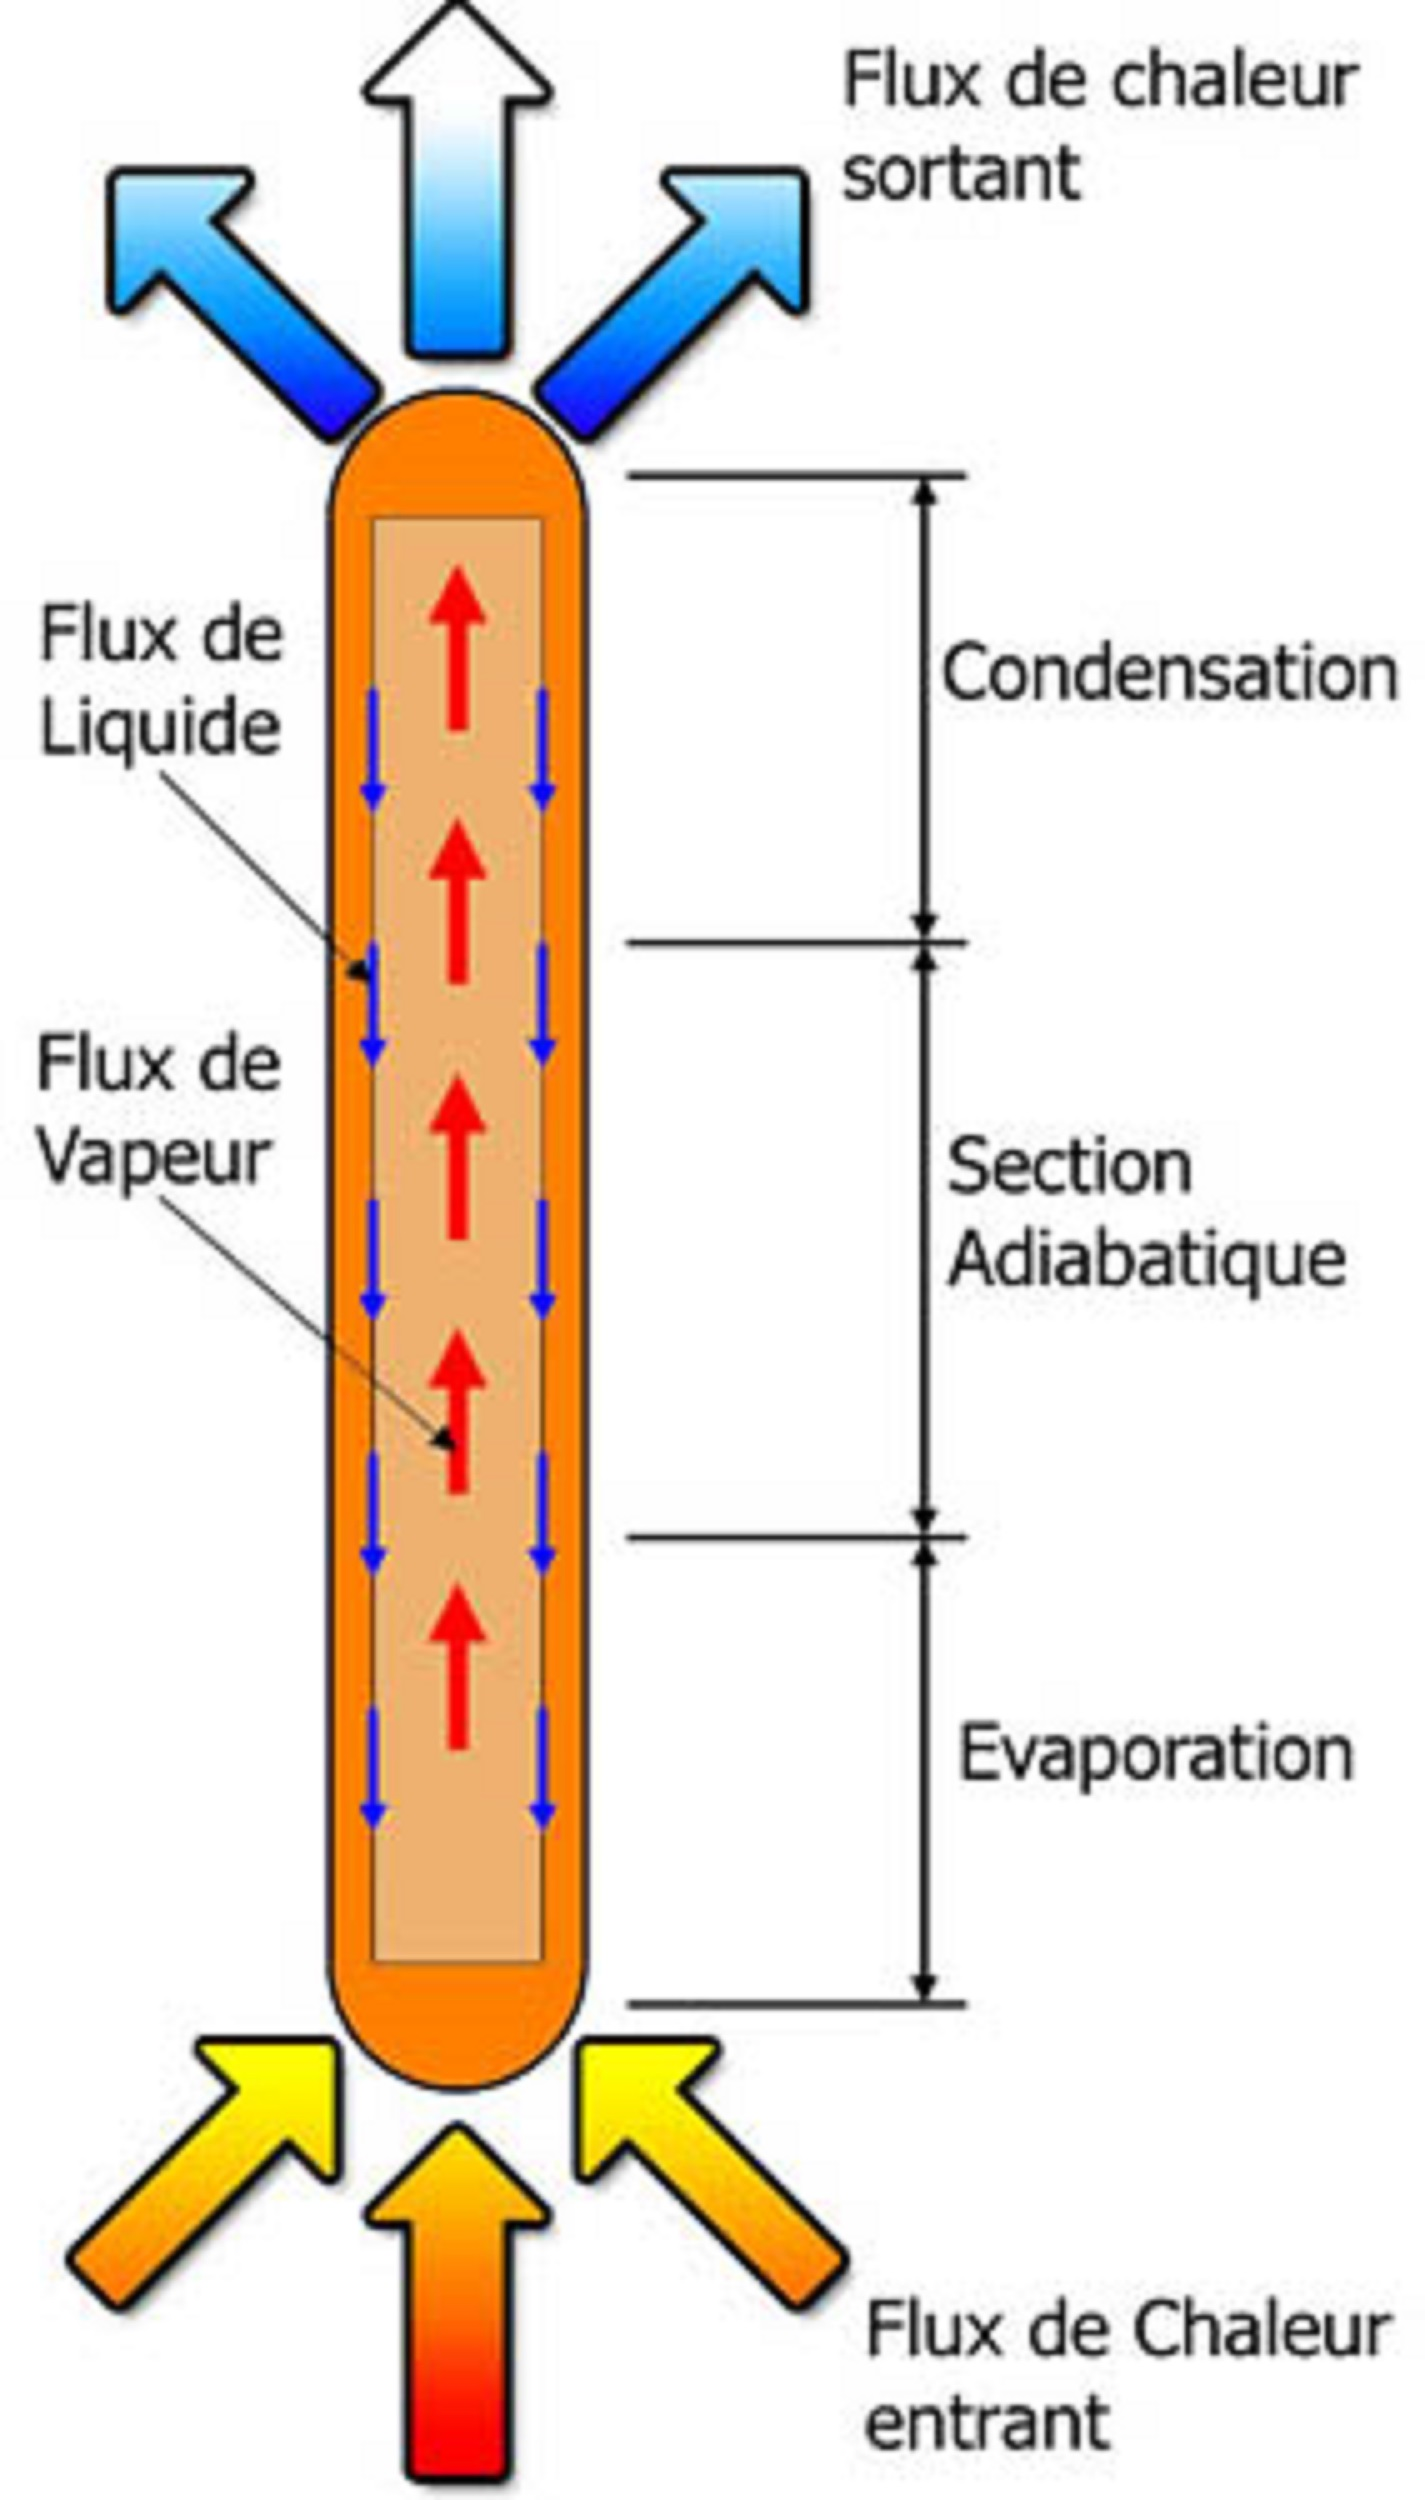
\includegraphics[scale=0.1]{3_1_caloduc.JPG}
\caption{Principe de fonctionnement des caloducs}
\end{center}
\end{figure}

	
%+photo des nouveaux raccords que je prendrai vendredi.

\end{document}